\section{Experiments}
\label{sec:experiments}

We evaluate PivotRL with three questions. First, under matched offline data, does replacing supervised fine-tuning (SFT) with PivotRL improve target-domain adaptation while better preserving held-out capability? Second, on SWE-Bench, where end-to-end reinforcement learning (E2E RL) is the most natural baseline, can PivotRL attain competitive accuracy with much lower online interaction? Third, are the two ingredients of the method---offline pivot filtering and functional reward---both necessary?

To answer these questions, we train PivotRL on four agentic domains: conversational tool use, software engineering, terminal control, and web browsing. The first comparison isolates the training objective under fixed prompts and expert trajectories; the SWE-Bench comparison isolates final accuracy versus rollout burden; and the ablations isolate state selection versus credit assignment. Across the four single-domain runs, PivotRL yields a larger average in-domain gain than same-data SFT (+14.11 vs.\ +9.94) while reducing average held-out/OOD change from $-9.48$ to $+0.20$. Unless otherwise stated, all experiments start from \texttt{Qwen3-30B-A3B-Thinking-2507}, use Nemo-RL \citep{nemo-rl} for optimization, and use Nemo-Gym \citep{nemo-gym} for environment rollouts. For every SFT--PivotRL comparison, the base model, prompts, and expert trajectories are matched exactly; only the training objective differs.

\subsection{Experimental questions and benchmarks}
\label{sec:exp_questions_benchmarks}

We evaluate PivotRL on four agentic benchmarks spanning the domains studied in this paper.

\begin{itemize}
  \item \textbf{$\tau^2$-Bench} \citep{barres2025tau2bench} evaluates conversational tool use in multi-turn customer-service environments. It contains three subsets: Retail and Airline \citep{yao2024taubench}, which primarily test agent tool use, and Telecom, which additionally includes user tool calls. We keep the user simulator fixed to \texttt{Qwen3-235B-A22B-Instruct-2507} in all evaluations.
  
  \item \textbf{SWE-Bench Verified} \citep{jimenez2024swebench} evaluates software-engineering agents on real GitHub issues that require understanding the problem, localizing the bug, and producing a correct patch. We use the verified subset of 500 tasks and evaluate with the OpenHands harness.

  \item \textbf{Terminal-Bench} \citep{tbench_2025} evaluates bash-terminal agents on tasks ranging from filesystem navigation and coding to system administration and more complex problem-solving. We evaluate on TBCore-v1.1 with the Terminus-2 harness.

  \item \textbf{BrowseComp} \citep{wei2025browsecompsimplechallengingbenchmark} evaluates web-search agents on difficult information-seeking questions that often require long trajectories with many search calls and nontrivial evidence synthesis.
\end{itemize}

Throughout this section, we call every extracted assistant turn a \emph{pivot candidate} and reserve the term \emph{pivot} for the offline-filtered subset used for PivotRL training. An \emph{action} is the full assistant completion at a model-call boundary, not an individual token. Depending on the benchmark, that completion may be a conversational tool-use turn, a coding-agent tool call, a bash command, or a search/browsing step. Natural-language-only assistant turns are also actions when the benchmark includes them. In the single-domain experiments, OOD change means the score difference relative to the base model on benchmarks outside the training domain. In the multi-domain experiment, the four agentic benchmarks are all training domains, so the remaining suite should be interpreted as held-out retention evaluations rather than strict OOD domains.

\subsection{Same-data comparison to SFT}
\label{sec:same_data_sft}

We first ask whether local verifier-based RL is a better post-training objective than behavior cloning when the data are held fixed. This is the cleanest comparison in the paper: SFT and PivotRL see the same prompts and expert trajectories, and the only difference is whether the model is trained to imitate the demonstrated continuation or to explore locally around selected pivots with domain verifier-based reward. Because SFT uses no online interaction and PivotRL uses only local one-turn or short partial rollouts, this comparison isolates the value of the objective under matched data; the direct rollout-burden comparison to full-trajectory RL is deferred to Section~\ref{sec:swe_e2e}.

\begin{table}[t]
\centering
\small
\begin{tabular}{lccccc}
\toprule
\textbf{Benchmark} & \textbf{Base} & \textbf{SFT} & \textbf{PivotRL} & \textbf{$\Delta$ vs Base} & \textbf{$\Delta$ vs SFT} \\
\midrule
$\tau^2$-Bench   & 44.35 & 58.44 & 63.81 & +19.46 & +5.37 \\
SWE-Verified     & 19.07 & 37.40 & 32.67 & +13.60 & -4.73 \\
Terminal-Bench   & 5.42  & 13.75 & 20.00 & +14.58 & +6.25 \\
BrowseComp       & 2.50  & 1.50  & 11.30 & +8.80  & +9.80 \\
\bottomrule
\end{tabular}
\caption{
Single-domain in-domain results under matched training data.
SFT and PivotRL use the same prompts and expert trajectories; only the training objective differs.
}
\label{tab:single_domain_main_results}
\end{table}

Table~\ref{tab:single_domain_main_results} answers the first question positively on average. PivotRL improves over the base model in all four training domains and achieves a larger average in-domain gain than same-data SFT (+14.11 vs.\ +9.94). It outperforms same-data SFT on $\tau^2$-Bench, Terminal-Bench, and BrowseComp.

We next evaluate held-out retention. For a model trained on one target domain, we treat the remaining benchmarks as held-out/OOD and report change relative to the base model. If PivotRL behaves more like on-policy RL than behavior cloning, it should remain closer to the base model outside the training domain.

\begin{table*}[t]
\centering
\small
\resizebox{\textwidth}{!}{%
\begin{tabular}{l c cc cc cc cc}
\toprule
\multirow{3}{*}{\textbf{Benchmark}} 
& \multirow{3}{*}{\textbf{Baseline}} 
& \multicolumn{8}{c}{\textbf{Training Domain (score + $\Delta$)}} \\
\cmidrule(lr){3-10}
& 
& \multicolumn{2}{c}{$\tau^2$} 
& \multicolumn{2}{c}{SWE} 
& \multicolumn{2}{c}{Terminal} 
& \multicolumn{2}{c}{BrowseComp} \\
\cmidrule(lr){3-4} \cmidrule(lr){5-6} \cmidrule(lr){7-8} \cmidrule(lr){9-10}
& Qwen3-30B 
& sft & rl 
& sft & rl 
& sft & rl 
& sft & rl \\
\midrule
\midrule

\textbf{Peak In-Domain} 
& -- 
& 58.44 (+14.09) & 63.81 (+19.46)
& 37.40 (+18.33) & 32.67 (+13.60)
& 13.75 (+8.33)  & 20.00 (+14.58)
& 1.50 (-1.00)   & 11.30 (+8.80) \\
\midrule

IFBench 
& 52.04 
& 44.42 (-7.62) & 53.29 (+1.25)
& 38.80 (-13.24) & 54.79 (+2.75)
& 24.77 (-27.27) & 49.47 (-2.57)
& 54.35 (+2.31)  & 53.89 (+1.85) \\

AIME25 
& 86.04 
& 76.25 (-9.79) & 85.63 (-0.41)
& 82.29 (-3.75)  & 85.00 (-1.04)
& 21.56 (-64.48) & 82.92 (-3.12)
& 85.21 (-0.83)  & 85.83 (-0.21) \\

MATH500 
& 98.05 
& 98.00 (-0.05) & 98.35 (+0.30)
& 98.30 (+0.25)  & 98.65 (+0.60)
& 63.55 (-34.50) & 98.00 (-0.05)
& 98.30 (+0.25)  & 98.40 (+0.35) \\

LiveCodeBench 
& 66.52 
& 64.98 (-1.54) & 66.96 (+0.44)
& 57.27 (-9.25)  & 66.96 (+0.44)
& 45.15 (-21.37) & 64.54 (-1.98)
& 67.62 (+1.10)  & 66.96 (+0.44) \\

Scicode 
& 36.83 
& 31.95 (-4.88) & 38.68 (+1.85)
& 24.85 (-11.98) & 39.87 (+3.04)
& 9.39 (-27.44)  & 39.13 (+2.30)
& 35.58 (-1.25)  & 37.28 (+0.45) \\

MMLU-Pro 
& 80.84 
& 79.81 (-1.03) & 81.31 (+0.47)
& 78.90 (-1.94)  & 81.13 (+0.29)
& 71.57 (-9.27)  & 80.85 (+0.01)
& 81.13 (+0.29)  & 81.31 (+0.47) \\

MMLU-ProX 
& 78.58 
& 74.31 (-4.27) & 78.92 (+0.34)
& 75.58 (-3.00)  & 78.81 (+0.23)
& 59.13 (-19.45) & 78.49 (-0.09)
& 76.68 (-1.90)  & 78.60 (+0.02) \\

WMT24++ 
& 36.97 
& 34.25 (-2.72) & 36.54 (-0.43)
& 35.69 (-1.28)  & 36.66 (-0.31)
& 6.31 (-30.66)  & 36.48 (-0.49)
& 33.18 (-3.79)  & 36.26 (-0.71) \\

\bottomrule
\end{tabular}%
}
\caption{
Held-out/OOD regression across four single-domain training runs.
Each cell shows score followed by per-task $\Delta$ relative to the Qwen3-30B baseline.
All RL--SFT comparisons use identical seed prompts and trajectories.
}
\label{tab:single_domain_ood_full}
\end{table*}

\begin{table}[t]
\centering
\small
\begin{tabular}{l c cc}
\toprule
\textbf{Evaluation} & \textbf{Baseline} & \textbf{Avg $\Delta$ SFT} & \textbf{Avg $\Delta$ RL} \\
\midrule
\textbf{In-Domain (Peak)} & -- & +9.94 & +14.11 \\
\midrule
IFBench        & 52.04 & -10.45 & +0.82 \\
AIME25         & 86.04 & -19.71 & -1.20 \\
MATH500        & 98.05 & -8.58  & +0.30 \\
LiveCodeBench  & 66.52 & -8.41  & -0.16 \\
Scicode        & 36.83 & -8.89  & +1.91 \\
MMLU-Pro       & 80.84 & -3.05  & +0.31 \\
MMLU-ProX      & 78.58 & -7.15  & +0.13 \\
WMT24++        & 36.97 & -9.59  & -0.49 \\
\midrule
\textbf{Avg OOD (All Benchmarks)} & 66.98 & -9.48 & +0.20 \\
\bottomrule
\end{tabular}
\caption{
Average performance change ($\Delta$) relative to the Qwen3-30B baseline across four single-domain training runs.
PivotRL achieves larger average in-domain gains while maintaining near-zero average held-out/OOD change, whereas same-data SFT exhibits substantial forgetting.
}
\label{tab:single_domain_ood_avg}
\end{table}

Tables~\ref{tab:single_domain_ood_full} and~\ref{tab:single_domain_ood_avg} show the clearest qualitative difference in the paper. Same-data SFT often improves the target domain but moves the policy far away from its starting distribution on unrelated tasks, producing an average held-out change of $-9.48$. PivotRL, by contrast, stays near the base model on the same evaluation suite, with average held-out change $+0.20$. The sharpest divergence appears after terminal-domain training: same-data SFT causes broad regression across IFBench, AIME25, MATH500, LiveCodeBench, Scicode, MMLU-Pro, MMLU-ProX, and WMT24++, whereas PivotRL remains much closer to baseline. Taken together with Table~\ref{tab:single_domain_main_results}, this is the main empirical pattern: same-data PivotRL usually matches or exceeds SFT on the target benchmark and preserves non-target capability far better.

\subsection{Comparison to end-to-end RL on SWE-Bench}
\label{sec:swe_e2e}

SWE-Bench is the stress test for the efficiency question because E2E RL is a particularly natural baseline: solving a GitHub issue requires long tool-using trajectories, and the final harness provides a clear end-to-end success signal. The question here is not whether PivotRL fully replaces E2E RL, but whether it recovers a large fraction of E2E RL's accuracy at much lower online cost, and whether it provides a useful warm start for subsequent E2E RL.

\begin{table}[t]
\centering
\small
\begin{tabular}{lccc}
\toprule
\textbf{Method} & \textbf{Score} & \textbf{Total Env. Actions} & \textbf{Training Regime} \\
\midrule
Base model & 19.07 & -- & none \\
Same-data SFT & 37.40 & offline only & behavior cloning \\
PivotRL & 32.67 & [PLACEHOLDER] & local turn-level RL \\
E2E RL & [PLACEHOLDER] & [PLACEHOLDER] & full-trajectory RL \\
PivotRL $\rightarrow$ E2E RL & [PLACEHOLDER] & [PLACEHOLDER] & local RL then full-trajectory RL \\
\bottomrule
\end{tabular}
\caption{
SWE-Bench comparison to end-to-end RL.
\textbf{Total Env. Actions} is the primary rollout-cost axis: the total number of environment actions executed during training, aggregated across all online rollouts.
}
\label{tab:swe_e2e}
\end{table}

All methods in Table~\ref{tab:swe_e2e} start from the same base model and are evaluated with the same OpenHands harness. The difference between PivotRL and E2E RL is therefore the training interaction pattern: PivotRL performs one-turn or short partial rollouts from offline-selected pivots, whereas E2E RL repeatedly executes full issue-solving trajectories. We use total environment actions as the main cost metric because it captures the quantity of online interaction in both regimes without mixing in unrelated implementation details.

This section is also where the current SWE local verifier should be interpreted most carefully. In the present setup, a SWE action is the next assistant tool call in the coding trace, and the local verifier matches tool-call names only. This is intentionally coarse: it rewards choosing the correct next \emph{kind} of operation at the pivot (for example, search, open, edit, or run) without attempting to score tool arguments or patch quality at every step. Final task correctness is still determined only by the full SWE-Bench evaluation harness. 

The final row, PivotRL $\rightarrow$ E2E RL, tests complementarity rather than substitution. [PLACEHOLDER -- If results are good, we can use PivotRL as a warm-start and combine orthogonally with E2E RL]

\subsection{Component ablations}
\label{sec:component_ablations}

We next answer the third question by separating state selection from local credit assignment. The naive baseline is obtained by sampling pivot candidates uniformly and using strict exact-match reward. PivotRL changes two things relative to that baseline: it filters to informative pivots offline, and it replaces strict exact matching with a functional verifier-based reward. The following ablations change one ingredient at a time.

\subsubsection{Pivot selection on $\tau^2$-Bench}
\label{sec:tau_pivot_ablation}

We use $\tau^2$-Bench as the main pivot-selection testbed because it is the lowest-cost environment in our suite and therefore supports controlled ablations at scale. Table~\ref{tab:tau_pivot_selection} compares three pivot datasets: random pivots, mixed-outcome pivots, and a stricter difficult mixed-outcome subset. The random-pivot baseline is the direct local-RL construction obtained by sampling pivot candidates uniformly, without offline filtering.

\begin{table*}[t]
\small
\centering
\setlength{\tabcolsep}{6pt}
\newcolumntype{F}{>{\centering\arraybackslash}p{0.8cm}}
\newcolumntype{C}{>{\centering\arraybackslash}p{0.8cm}}
\begin{tabular}{l|F|F|C|C}
\toprule
& \multicolumn{1}{c|}{\textbf{$\tau^2$-Airline}}
& \multicolumn{1}{c|}{\textbf{$\tau^2$-Retail}}
& \multicolumn{1}{c|}{\textbf{$\tau^2$-Telecom}}
& \multicolumn{1}{c}{\textbf{$\tau^2$-Average}} \\
\midrule
gpt-oss-120b-high
& 55.33 & 58.19 & 67.20 & 60.24 \\
gpt-oss-20b-high
& 43.33 & 50.20 & 52.63 & 48.72 \\
Qwen3-235B-A22B-Thinking-2507
& 50.00 & 66.08 & 46.78 & 54.29 \\
\midrule
Qwen3-30B-A3B-Thinking-2507
& 50.00 & 54.39 & 28.65 & 44.35 \\
\hdashline
Qwen + SFT
& 51.33 & 58.19 & 65.79 & 58.44 \\
Qwen + Random Pivots
& 58.00 & 63.74 & 57.31 & 59.68 \\
Qwen + Mixed-Outcome Pivots
& 61.33 & 66.08 & 56.73 & 61.38 \\
Qwen + Difficult Mixed-Outcome Pivots
& 58.67 & 69.01 & 63.74 & 63.81 \\
\bottomrule
\end{tabular}
\caption{
Effect of pivot selection on $\tau^2$-Bench.
Best checkpoint over training.
Random pivots improve over the base model, mixed-outcome pivots improve further, and difficult mixed-outcome pivots perform best.
}
\label{tab:tau_pivot_selection}
\end{table*}

Table~\ref{tab:tau_pivot_selection} shows a monotonic benefit from better state selection. Random pivots already improve over the base model and slightly exceed same-data SFT, which confirms that converting demonstrations into local RL data is useful. However, offline filtering matters: keeping only mixed-outcome turns raises performance further, and restricting to the harder mixed-outcome subset yields the best result, 63.81. This is exactly the regime we expect from Proposition~\ref{prop:mixed}: states that still exhibit both success and failure under local sampling continue to produce informative normalized updates.

\begin{figure}[t]
    \centering
    \begin{minipage}{0.48\textwidth}
        \centering
        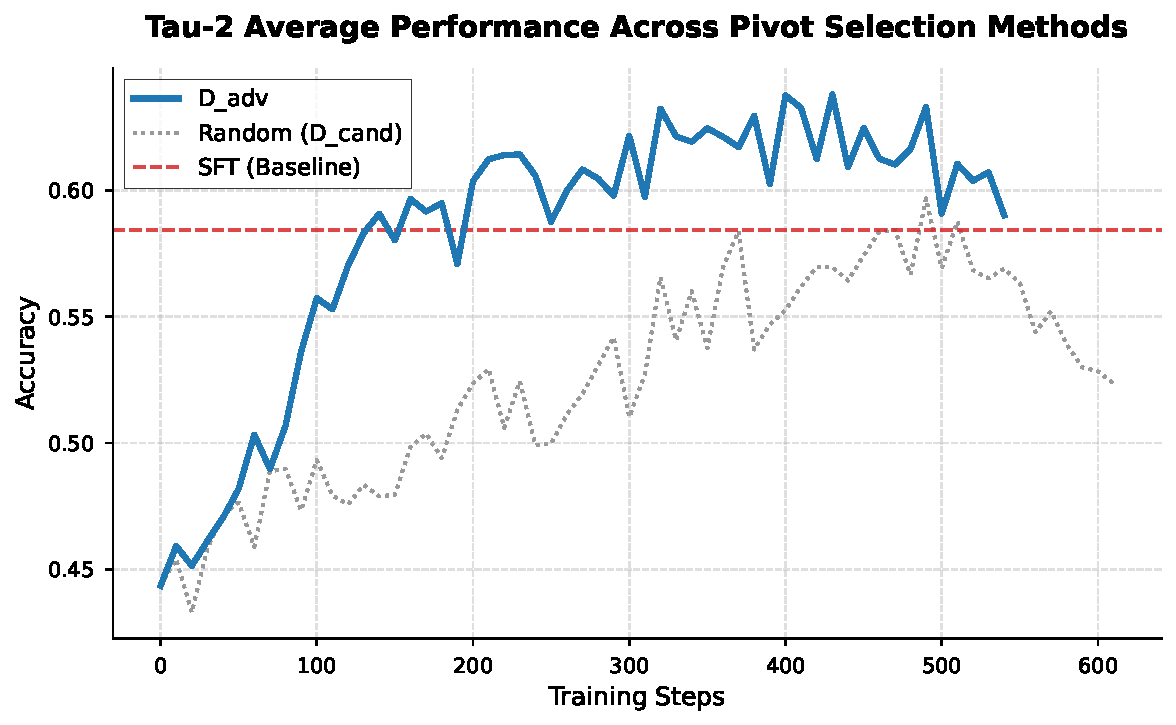
\includegraphics[width=\linewidth]{figures/main_average_validation.pdf}
        \caption{$\tau^2$-Bench accuracy over RL training. Difficult mixed-outcome pivots yield the strongest optimization and outperform same-data SFT.}
        \label{fig:tau_pivot_selection_acc}
    \end{minipage}
    \hfill
    \begin{minipage}{0.48\textwidth}
        \centering
        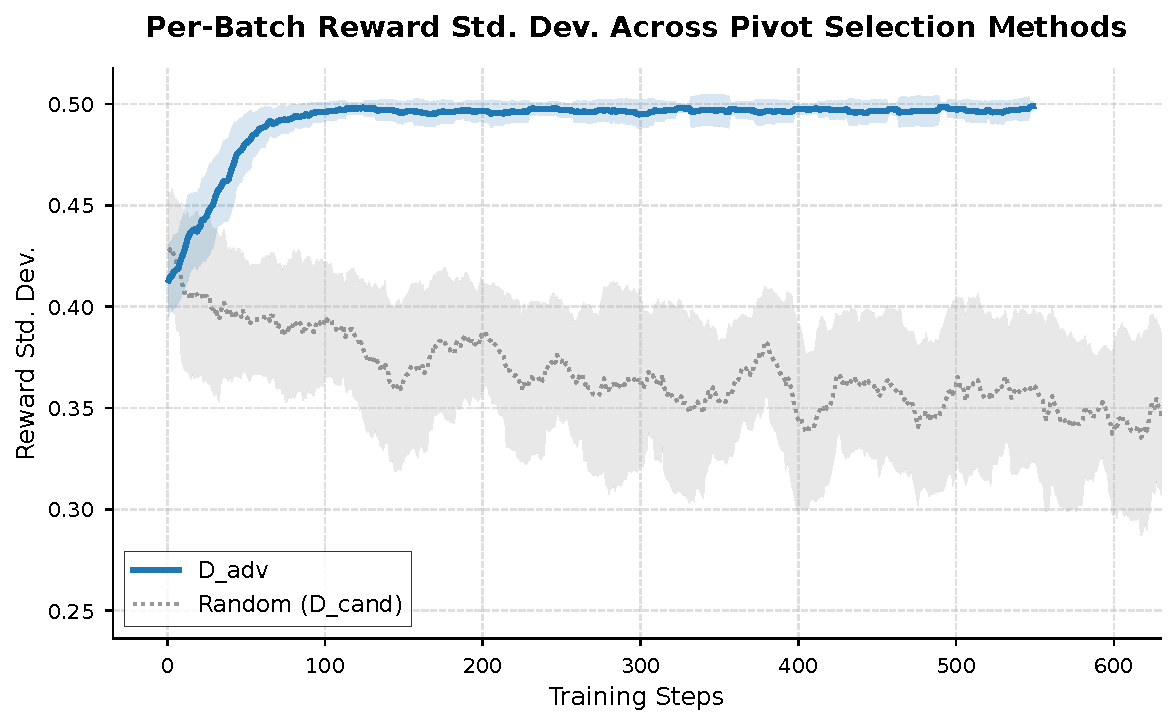
\includegraphics[width=\linewidth]{figures/tau_reward_stddev.pdf}
        \caption{$\tau^2$-Bench reward standard deviation during RL training. More selective pivot sets maintain higher reward variance and therefore more informative local updates.}
        \label{fig:tau_reward_std}
    \end{minipage}
\end{figure}

\begin{figure*}[t]
    \centering
    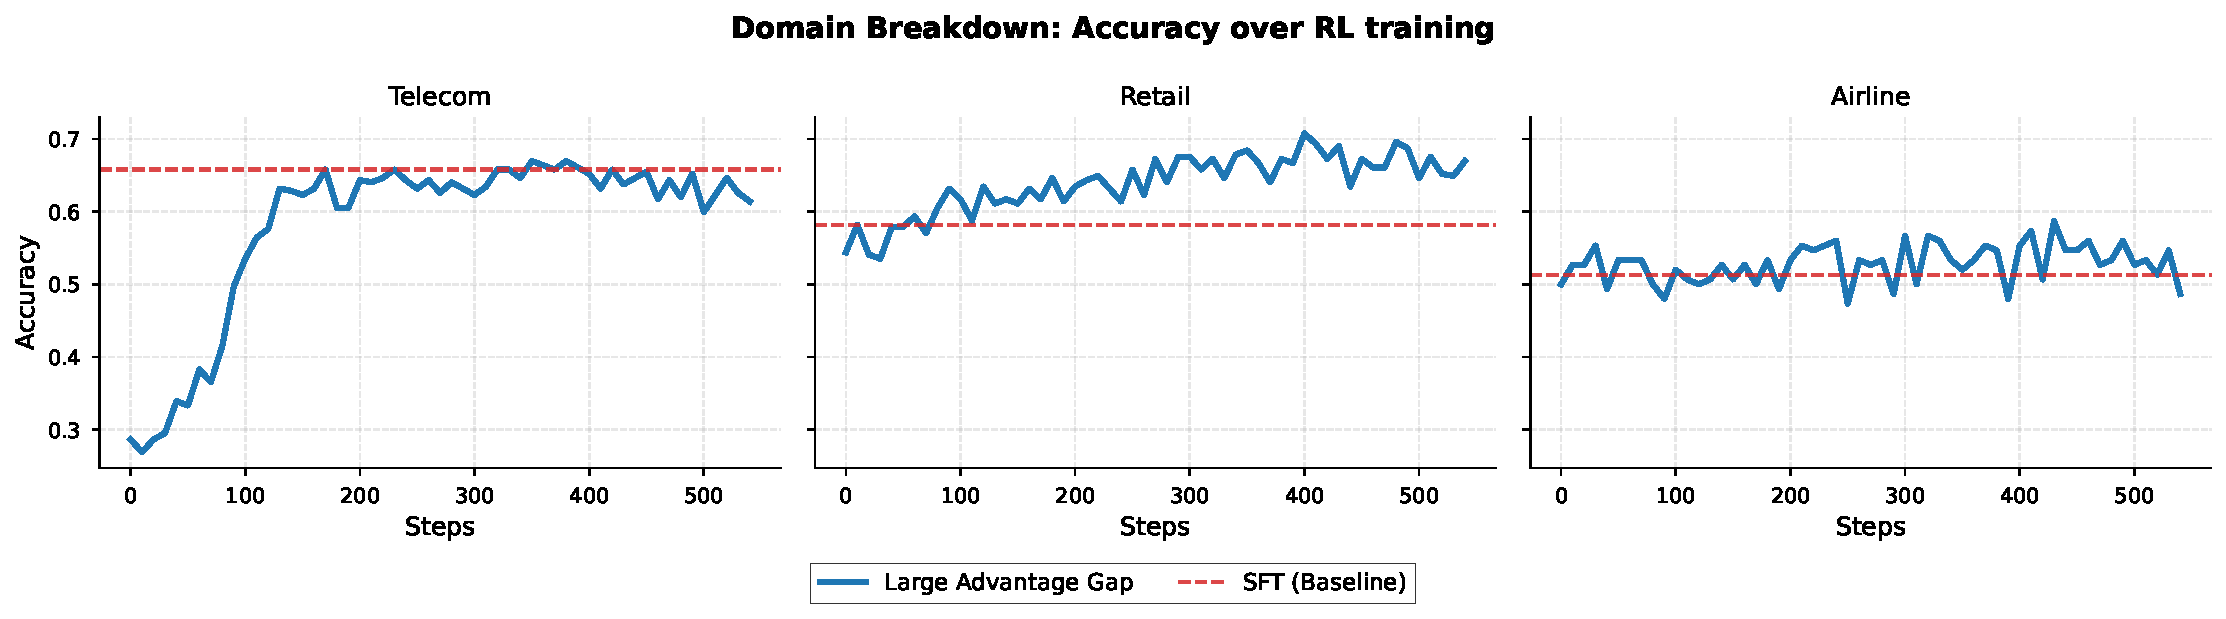
\includegraphics[width=1.0\textwidth]{figures/main_per_domain_validation_difficulty.pdf}
    \caption{Per-domain $\tau^2$-Bench accuracy over RL training for the difficult mixed-outcome pivot set. From left to right: Telecom, Retail, Airline.}
    \label{fig:tau_domain_breakdown}
\end{figure*}

Figures~\ref{fig:tau_pivot_selection_acc} and~\ref{fig:tau_reward_std} show why the filtered pivot sets work better. Under random sampling, per-batch reward variance collapses quickly, indicating that many sampled turns no longer generate a useful advantage signal. The mixed-outcome and difficult mixed-outcome pivot sets preserve higher reward variance deeper into training and also optimize to higher validation accuracy. Figure~\ref{fig:tau_domain_breakdown} shows the per-domain improvement for the strongest pivot set.

\subsubsection{Functional reward and joint 2$\times$2 ablation}
\label{sec:joint_ablation}

We next cross the two design choices directly:
\[
\{\text{random pivots},\ \text{informative pivots}\}
\quad \times \quad
\{\text{strict reward},\ \text{functional reward}\}.
\]
Random pivots + strict reward is the direct local-RL baseline from Section~\ref{sec:prelim}; full PivotRL corresponds to informative pivots + functional reward.

\begin{table}[t]
\centering
\small
\begin{tabular}{lcc}
\toprule
\textbf{Pivot Set} & \textbf{Strict Reward} & \textbf{Functional Reward} \\
\midrule
Random pivots & [PLACEHOLDER] & [PLACEHOLDER] \\
Informative pivots & [PLACEHOLDER] & [PLACEHOLDER] \\
\bottomrule
\end{tabular}
\caption{
Joint ablation of state selection and reward design.
Moving across a row changes only the reward; moving down a column changes only the pivot set.
The full method corresponds to informative pivots with functional reward.
}
\label{tab:joint_component_ablation}
\end{table}

Table~\ref{tab:joint_component_ablation} should be read as a clean decomposition of the main gain. If functional reward helps when the pivot set is fixed, then exact matching is too sparse as local supervision. If informative pivots help when the reward is fixed, then the bottleneck is not only reward design but also where the online exploration budget is spent. The full method is expected to dominate because it improves both axes simultaneously.


\subsection{Benchmark-specific training details}
\label{sec:benchmark_specific_details}

In all four domains, pivot candidates are extracted once from the demonstration traces, profiled offline, and filtered before RL training; training then samples only from the retained pivot set. We summarize the domain-specific action units, data construction, and local verifiers here. Full profiling details and hyperparameters are deferred to the appendix.

\paragraph{$\tau^2$-Bench.}
We curate an SFT trajectory dataset of 281{,}774 trajectories across 838 domains using a synthetic data-generation pipeline similar to ToolAce \citep{liu2025toolacewinningpointsllm}, Kimi-K2 \citep{kimiteam2025kimik2openagentic}, and DeepSeek-V3.2 \citep{deepseekai2025deepseekv32pushingfrontieropen}. We train on top of \texttt{Qwen3-30B-A3B-Thinking-2507}. Every assistant turn in the trace is first treated as a pivot candidate. In this domain, an action is the full assistant turn at the model-call boundary, which may contain natural language, tool calls, or both. We then evaluate random, mixed-outcome, and difficult mixed-outcome pivot sets as described in Section~\ref{sec:pivotrl_method}.

\paragraph{Terminal-Bench.}
We collect resolved trajectories from \texttt{Qwen/Qwen3-Coder-480B-A35B-Instruct} and \texttt{moonshotai/Kimi-K2-Instruct} using the Terminus-1 and Terminus-2 agents. Every assistant bash action is treated as a pivot candidate, and an action in this domain is the next bash command produced at the model-call boundary. We start from the difficult mixed-outcome set $\mathcal{D}_{\mathrm{adv}}$, with an additional command-deduplication step to improve diversity. The final dataset contains approximately 20{,}000 samples. The local verifier asks whether the sampled command is locally interchangeable with the demonstrated command: it combines output-schema validation, normalized string similarity, and equivalence-based LLM-as-judge scoring over the command and its immediate effect.

\paragraph{SWE-Bench Verified.}
We use an internal trajectory dataset generated with OpenHands \citep{wang2025openhandsopenplatformai}, OpenCode \citep{opencode}, and Codex \citep{openaicodex_software} on tasks including SWE-Gym \citep{pan2025trainingsoftwareengineeringagents} and R2E-Gym \citep{jain2025r2egymproceduralenvironmentshybrid}, using \texttt{MiniMaxAI/MiniMax-M2.5} \citep{minimax2026m25}. We evaluate mean@3 with the OpenHands harness. Every non-error tool-call action is treated as a pivot candidate, and an action in this domain is the next assistant tool call in the coding trace. Filtering to $\mathcal{D}_{\mathrm{adv}}$ yields a final training set of 87{,}718 samples. In the current experiments, the local verifier matches tool-call names only. This is a deliberately coarse local signal: it checks whether the model selected the correct next \emph{kind} of operation at the pivot, without attempting to score tool arguments or patch quality at every turn. Final task success is still determined only by the full SWE-Bench evaluation harness.

\paragraph{BrowseComp.}
We start from a multi-hop question-answer dataset and use an online search engine together with \texttt{DeepSeek-V3.2} to generate browsing trajectories. Each search-related assistant step at a model-call boundary is treated as a pivot candidate; in this domain, an action is the next browsing step, such as issuing a search, opening a result, or taking the next evidence-gathering action. The final dataset contains 13{,}215 samples. Because this dataset is comparatively small, we use random filtering ($\mathcal{D}_{\mathrm{random}}$) rather than the more selective pivot sets.